\documentclass[final,12pt,3p]{elsarticle}

%% Use the options 1p,twocolumn; 3p; 3p,twocolumn; 5p; or 5p,twocolumn
%% \documentclass[final,3p,times]{elsarticle}
%% \documentclass[final,3p,times,twocolumn]{elsarticle}

%% Packages
\usepackage{amssymb}
\usepackage{amsthm}
\usepackage{float}
\usepackage{amsmath}
\usepackage{xcolor}
\usepackage{subcaption}
\usepackage{dsfont}

%% Code syntax
\def\code#1{\texttt{#1}}

%% Start
\journal{Dr.Frederic Godin, Concordia University}

\begin{document}

\begin{frontmatter}
    \title{Various Reinforcement Learning Algorithms to Solve Grid World}

    \author[label1]{Matteo Esposito}
    \ead{ds.mesposito@gmail.com, ID:40024121}
    \author[label1]{William Ngo}
    \ead{ngowilliam96@gmail.com, ID:40031586}
    \author[label1]{Spyros Orfanos}
    \ead{spyros.orfanos1@gmail.com, ID:40032280}
    \address[label1]{Concordia University, Montreal, Quebec}

    \begin{abstract}
        Reinforcement Learning (RL) is widely used in different research areas to tackle problems such as resource management in computers\cite{tds}, traffic light control\cite{tds}, and playing games like chess\cite{deepmind} at a super-human level. In this project, we tackle the problem of solving a two- dimensional maze given a specific starting point. To accomplish this, three different policies were developed using RL algorithms known as SARSA, Q-Learning, and n-step SARSA.  Each learning method has its own theoretical tradeoffs, which we compare by evaluating the average training time per single run, average number of episodes until they reach optimality, and scalability by testing the algorithms on two different sized mazes. We conclude that Q-Learning is the best suited approach for this problem since in both of our mazes, we observed consistently faster convergence to the optimal return and execution times.
    \end{abstract}
    
\end{frontmatter}

\section{Introduction}

Our project, commonly referred to as “Grid World”, tackles the problem of exiting a two-dimensional maze. This problem consists of a starting point, an exit point, and a board in which the agent (player) can take actions to move up, down, left or right. This is quite a simple task for a human as one can simply inspect the entirety of the maze and, at a glance, deduce an exit strategy. However, a machine cannot readily “see” the maze or “think” of actions to take, so how can it learn to solve a maze?
\par
To allow a machine to “understand” the problem at hand, we must first reformulate the problem into something it can understand: a sequential decision problem. A sequential decision problem consists of a set of states, a set of actions, and an objective. By formulating the problem in such a way, we may use Reinforcement Learning (RL) techniques to solve the problem. 
\par
RL is learning what to do: how to map situations to actions so as to maximize some long-term reward. To do this, a numerical return is designed such that when maximized, the objective of the problem should be met.\cite{godin} In other words, RL is all about discovering the best action given your current state.
\par
The goal of this project is to compare the rate of convergence of the estimated value function at the starting position, $\hat{V}_{*}(S_0)$, to the optimal policy’s value function at the starting position, $V_{*}(S_0)$, of three RL methods: SARSA, Q-Learning, and n-step SARSA. This is measured in three ways: number of episodes until convergence to $V_{*}(S_0)$, run time of the algorithms, and how the algorithms scale to a larger maze. (See figures 1 and 2 for the mazes we considered for this project.) 

\section{Problem Description}

As described above, “Grid World” is a sequential decision problem as the set of states is the possible positions in the maze, the set of actions is deciding which direction to go and the objective is to find the exit of the maze in the shortest amount of steps, given a starting point and the exit point.

\begin{figure}[H]
    \centering
    \begin{minipage}{.5\textwidth}
      \centering
      \caption{Form of maze 1}
      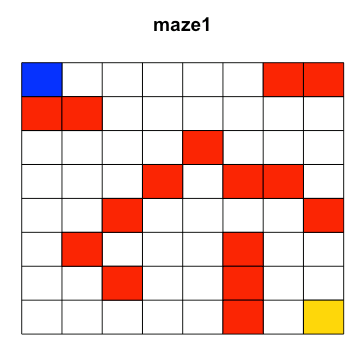
\includegraphics[width=8cm]{figures/EmptyMaze1Map.png}
    \end{minipage}%
    \begin{minipage}{.5\textwidth}
      \centering
      \caption{Form of maze 2}
      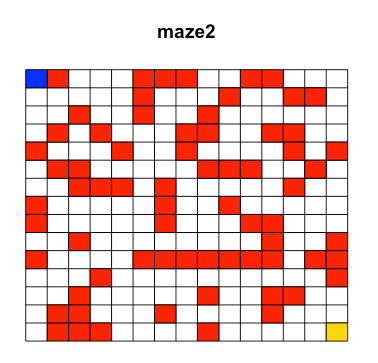
\includegraphics[width=8cm]{figures/EmptyMaze2Map.png}
    \end{minipage}
\end{figure}

\section{Analyses}

\subsection{Implementation - Code}
\vspace{12pt}

We would like to briefly comment on the structure of our code. The project can be run entirely from \code{main.R}. The environment of the maze was built using object-oriented programming, which was done with the R6 package. Object-oriented programming was a core concept in the design of our environment and our code as we wanted each script to do achieve specific task. By doing this, the script that generates the environment can be used for future tasks at hand. In \code{main.R} all of our algorithms are called (by means of the \code{source()} function) and with them, average runtimes, optimal action plots and average return plots are output. 

\subsection{Environment}
\vspace{12pt}

Here, the set of states consists of all valid board positions $(x,y)$ where $x \in \{1,2,\ldots, \; nrow\}$ and $y \in \{1,2,\ldots, \; ncol\}$. The set of actions consists of moving $\{\text{Right} \; (action = 1), \; \text{Down} \; (a = 2), \; \text{Left} \; (a = 3)$ $ \; \text{or} \; \text{Up} \; (a = 4)\}$ where the objective is to find the exit of the maze.
\par
To implement our maze, we create an m-by-n matrix that stores the values 0, 1 and 10. These three denote a valid space, a wall and an exit tile, respectively. The starting point of the agent is defined in the main script as the variable “ratStartingPosition”. This was designed in a manner in which we could easily modify the characteristics of the maze by simply modifying one or two variables. Through the use of object-oriented programming and the R6 package, we can access and modify many properties of our maze object.

For every action we assign a reward strictly dependent on the environment (set of states), with the following structure:

\begin{itemize}
    \item Reward attributed to hitting a wall - denoted as a red tile, or going beyond the border = -0.75 
    \item Reward attributed to revisiting a previously seen tile = -0.30
    \item Reward attributed to visiting a new, unseen tile that isn't the exit tile = -0.05 
    \item Reward attributed to visiting the exit tile - denoted as a yellow tile = 5 
\end{itemize}

Note that if the agent attempts to hit a wall or move beyond the bounds of the maze, then it stays in its current position and is attributed a reward of -0.75. The design of our rewards should effectively discourage the agent from wandering around aimlessly and encourage the agent to explore unseen states, which possibly lead to the exit. More information regarding the choice of rewards can be found in Appendix B. 

\par
Given the structure of our test mazes, the optimal return when starting in the upper-left corner is $G_0 = 3.85$ for maze 1 and 3.55 for maze 2. These will be denoted as the orange convergence asymptote in the average return plots presented in the following section.

\vskip 0.1in
\underline{Note:} All plots and future references represent runs that have been performed in the maze 1 environment unless stated otherwise.


\subsection{Statespace}
\vspace{12pt}

To simplify the RL algorithms, we consider the bijective mapping $f: \mathbb{N}^2 \rightarrow \mathbb{N}$ which maps valid board positions (x,y) to states (s). The mapping is as follows: the upper-left most corner is mapped to a value of 1 (referred to as state 0). Then, moving right along the first row, the next valid board position is mapped to the next natural number. Once all board positions in a given row are mapped to (s), we apply the same logic to the next row, until we have mapped all valid board positions. 

\vspace{12pt}
\subsubsection{Random Policy}
\vspace{12pt}

Before running any learning algorithm, we evaluated the performance of a policy that selects actions at random. As expected, this policy performs extremely poorly: out of 10000 episodes, only $\sim$11\% of the episodes were able to find the exit within 400 moves, and for the episodes that ended, the average return is much lower than that of the optimal return. The results are summarized below.

\begin{table}[H]
    \centering
    \caption{Results of random policy after 10000 episodes}
    \begin{tabular}{|c|c|}
        \hline
        Number of episodes that ended & Average Return of the policies that ended \\ \hline
        1075 & -115.569 \\ \hline
    \end{tabular}
    \caption*{Using the random policy algorithm, out of 10000 episodes only 10.75\% of all episodes exit the maze successfully/terminate within 400 steps, yielding an average reward of -115.596.}
\end{table}

\subsection{Algorithms}
\vspace{12pt}

Here we describe the theoretical backgrounds and state-action value update rules of the three approaches we considered. Note that all of our algorithms use $\varepsilon$-greedy policies, where the agent takes the greedy action (i.e., the agent's percieved optimal action) with probability 1 - $\varepsilon$, and takes a random, exploratory, action with probability $\varepsilon$. Also note that when implementing each algorithm we set $\alpha = 0.1$ and  $\gamma = 1$. 

\subsubsection{SARSA}
\vspace{12pt}

Our first RL algorithm is the SARSA (State-Action-Reward-State-Action) method. The SARSA method is an on-policy temporal difference control method. It enables the agent to update the state-action value function, $Q_{\pi}(s,a)$, after every action taken when following a given policy $\pi$. Its update rule is defined as follows:

\begin{align*}
    Q_{t+1}(S_t,A_t) \leftarrow Q_{t}(S_t,A_t) + \alpha[R_{t+1} + \gamma Q_t(S_{t+1},A_{t+1}) - Q_t(S_t,A_t)]
\end{align*}

\subsubsection{Q-Learning}
\vspace{12pt}

Q-Learning is another temporal difference control policy and is usually used as an off-policy method. Here, we instead use it as an on-policy method by updating the $\varepsilon$-greedy policy based on our estimate of Q(S,A). 

\begin{align*}
    Q_{t+1}(S_t,A_t) \leftarrow Q_{t}(S_t,A_t) + \alpha[R_{t+1} + \gamma\max_{a}Q_t(S_{t+1},A_{t+1}) - Q_t(S_t,A_t)]
\end{align*}

\subsubsection{n-Step SARSA}
\vspace{12pt}

Finally, the n-step SARSA method is considered. It is a variation of the aforementioned SARSA algortihm as it uses n-many rewards to update the estimate of $Q(S, A)$. It is implemented as follows:

\begin{align*}
    Q_{t+n}(S_t, A_t) &= Q_{t+n-1}(S_t, A_t) + \alpha[G_{t:t+n} - Q_{t+n-1}(S_t, A_t)] \\
    Q_{t+n}(s, a) &= Q_{t+n-1}(s, a) \quad \forall (s, a) \neq (S_t, A_t)
\end{align*}
\begin{align*}
    G_{t:t+n} = \sum_{j=1}^{\min(n, \tilde{T}_{I(t)}-t)}\gamma^{j-1}R_{t+j} + \mathds{1}_{\{t+n \leq \tilde{T}_{I(t)}\}} \gamma^nV_{t+n-1}(S_{t+n})
\end{align*}


\subsection{Considerations: Epsilon Selection}
\vspace{12pt}

Since all of our RL algorithms involve on-policy methods, the policies require exploration; however, this means the policy will converge to an $\varepsilon$-greedy policy. This presents a challenge, as we know that the optimal policy is deterministic. In order to have convergence to a deterministic policy, we explored different choices of epsilon, namely epsilons that were decreasing as the policy improved after each episode.

\par
We tested multiple epsilon update functions, and present the results from our Q-Learning algorithm below. As illustrated in the following figure, update rule $0.4/n$ performed quite poorly, most likely because it did not allow the agent enough time to explore at the start of the run. Next, we see that the log update rule and the exponentially decaying update rule outperform the constant epsilon in two ways. Firstly, the policy improved much faster, and secondly, the episode returns plateau at 3.85 as desired, unlike the constant epsilon policy which often dips below 3.85 due to taking exploratory actions. A possible explanation for the improvement is that these update rules, especially the exponentially decaying update rule, allowed for more exploration at the beginning of the run, when exploration is essential, and then progressively explored less, exploiting the optimal action.

\begin{figure}[H]
    \centering
    \caption{Q-Learning returns under various $\varepsilon$-update rules.}
    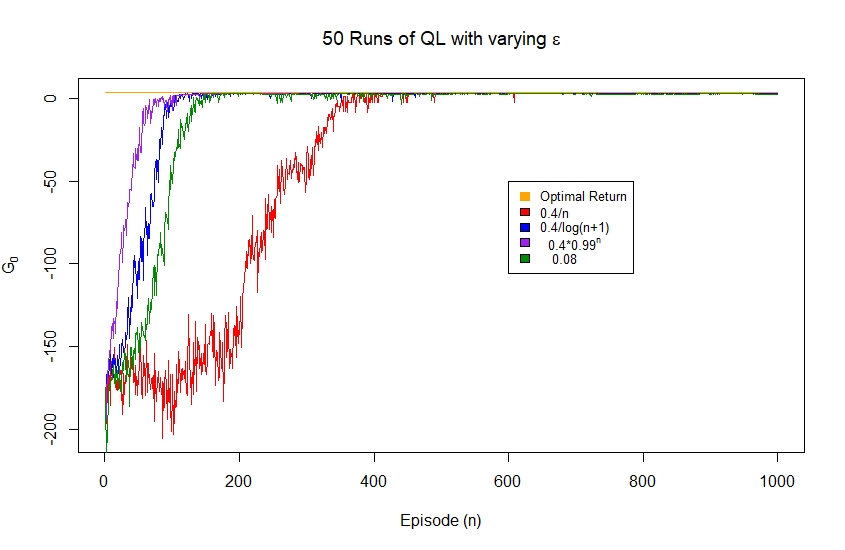
\includegraphics[width=13cm]{figures/VaryingEpsilon.jpeg}
\end{figure}

\begin{table}[H]
    \centering
    \caption{Varying epsilon approaches runtime analysis}
    \begin{tabular}{|c|c|c|}
        \hline
        \textbf{$\varepsilon_n$} & \textbf{Average \# Episodes Before Convergence} & \textbf{Runtime (mins/ep)} \\ \hline
        $\frac{0.4}{n}$ & $\sim$450 & $\sim$0.189 \\ \hline
        $\frac{0.4}{\log(n+1)}$ & $\sim$180 & $\sim$0.087 \\ \hline
        $0.4(0.99)^n$ & $\sim$120 & $\sim$0.073 \\ \hline
        $0.08$ & $\sim$200 & $\sim$0.109 \\ \hline
    \end{tabular}
\end{table}

\vspace{12pt}
\underline{Note:} The reported runtime averages are hardware dependent.

\subsection{Consideration: Bias vs. Variance Tradeoff}
\vspace{12pt}

Another consideration of any machine learning project is the bias-variance tradeoff. Since we are only dealing with TD (temporal difference) methods, we will only speak about the bias-variance present in these types of reinforcement leaning algorithms. Generally speaking, TD methods have lower variance but have higher bias compared to Monte-Carlo method. The lower variance is due to the fact that in the update equation for the value function of TD methods, the term/target value  $R_{t+1} + \gamma V_{\pi}(S_{t+1})$ shows that the state-value update utilizes only the immediate future reward while in contrast to the Monte Carlo method, which have target value $G_t = R_{t+1} + \gamma R_{t+2} + \ldots$, which clearly depend on a greater number of rewards.
\par
The presence of bias in the TD methods is due to the fact that the initial value function estimate is being used to update our value function estimate. It is worth noting that even though TD methods are biased, the bias is exponentially decaying thus asymptotically it is not an issue.
\par
n-Step SARSA is a method in which we can control the bias-variance tradeoff as the value function is updated using the next n-many rewards. The higher the n, the more rewards we utilize to update the value function and thus higher variance, vice-versa, the lower the n, the lower the variance but a higher bias is incurred.
\par
The concept of bias-variance tradeoff is a theoretical view of these learning methods but to know which learning method is best for a given problem we have to implement them and see which performs the best. Before comparing the different learning algorithms between each other, we first vary the “n” in n-Step SARSA to determine which one seems to be performs the best. We ran and compared 5,10 and 15 step SARSA implementations on our first 8x8 maze and observed the following results:

\begin{figure}[H]
    \centering
    \caption{Comparison of n-Step SARSA algorithms by return $G_0$ at different n-values with exponentially decaying $\varepsilon$ values.}
    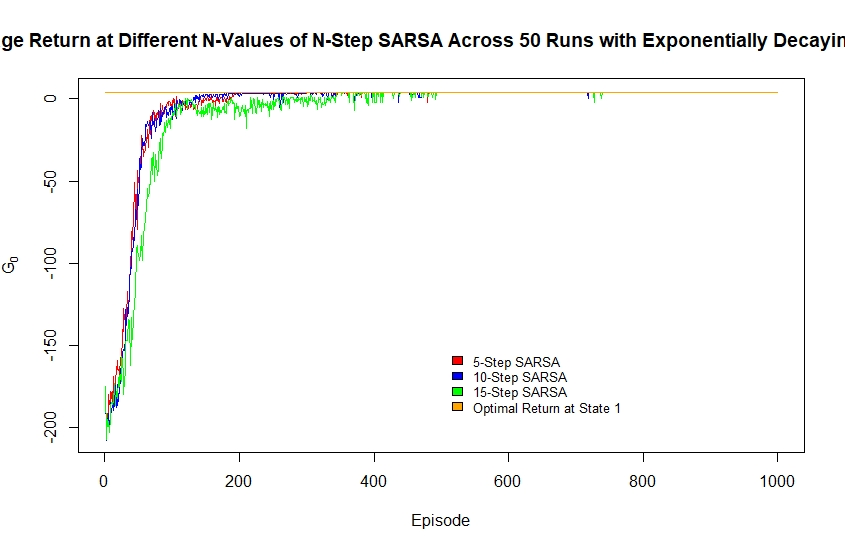
\includegraphics[trim=0 0 0 1.5cm, clip, width=14cm]{figures/5StepVS10StepVS15Step.jpeg}
\end{figure}

From the following figure we can conclude that there is no significant discrepancy between 5-step and 10-step SARSA whereas 15-step SARSA is less suited to our problem considering all 3 convergence rates. 5-step or 10-step is clearly better for this problem. We decided to use 10-step SARSA in all future analyses/plots.

\subsection{Maze 1 Results}

\begin{figure}[H]
    \centering
    \caption{Maze 1 returns}
    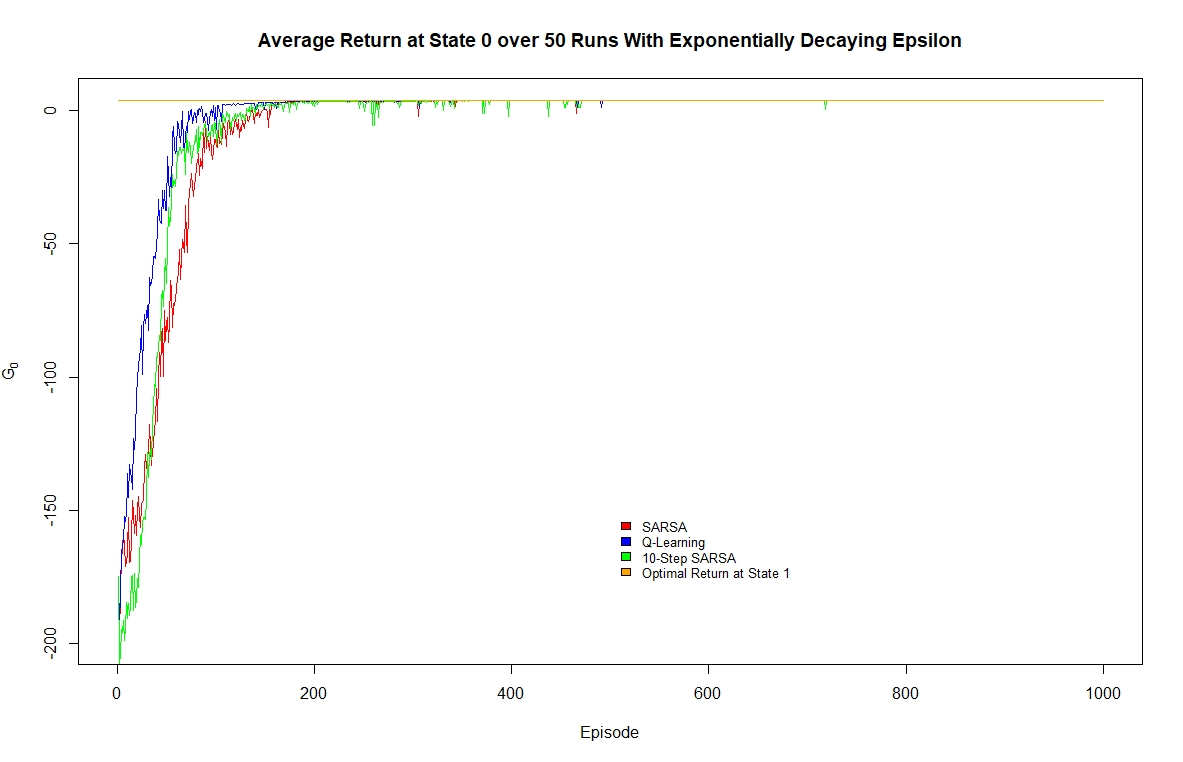
\includegraphics[width=14cm]{figures/Maze1.jpeg}
\end{figure}

\begin{table}[H]
    \centering
    \caption{Maze 1 runtime analysis}
    \begin{tabular}{|c|c|c|}
        \hline
        \textbf{Algorithm} & \textbf{Average \# Episodes Before Convergence} & \textbf{Runtime (mins/run)} \\ \hline
        SARSA & $\sim$200 & $\sim$0.085 \\ \hline
        Q-Learning & $\sim$150 & $\sim$0.075 \\ \hline
        n-Step SARSA & $\sim$200 & $\sim$0.094 \\ \hline
    \end{tabular}
\end{table}

We observe that Q-Learning converges faster than SARSA and 10-step SARSA. It converges in roughly 3/4 the number of episodes and has a per episode runtime which is quicker than that of the SARSA algorithms. We can observe that the average runtime is proportional to the average number of episodes before convergence because past a certain point, when the agent selects the greedy action, it will select the optimal action and thus an episode would terminate quickly.

\begin{figure}[H]
    \centering
    \caption{Optimal actions on maze 1 using SARSA}
    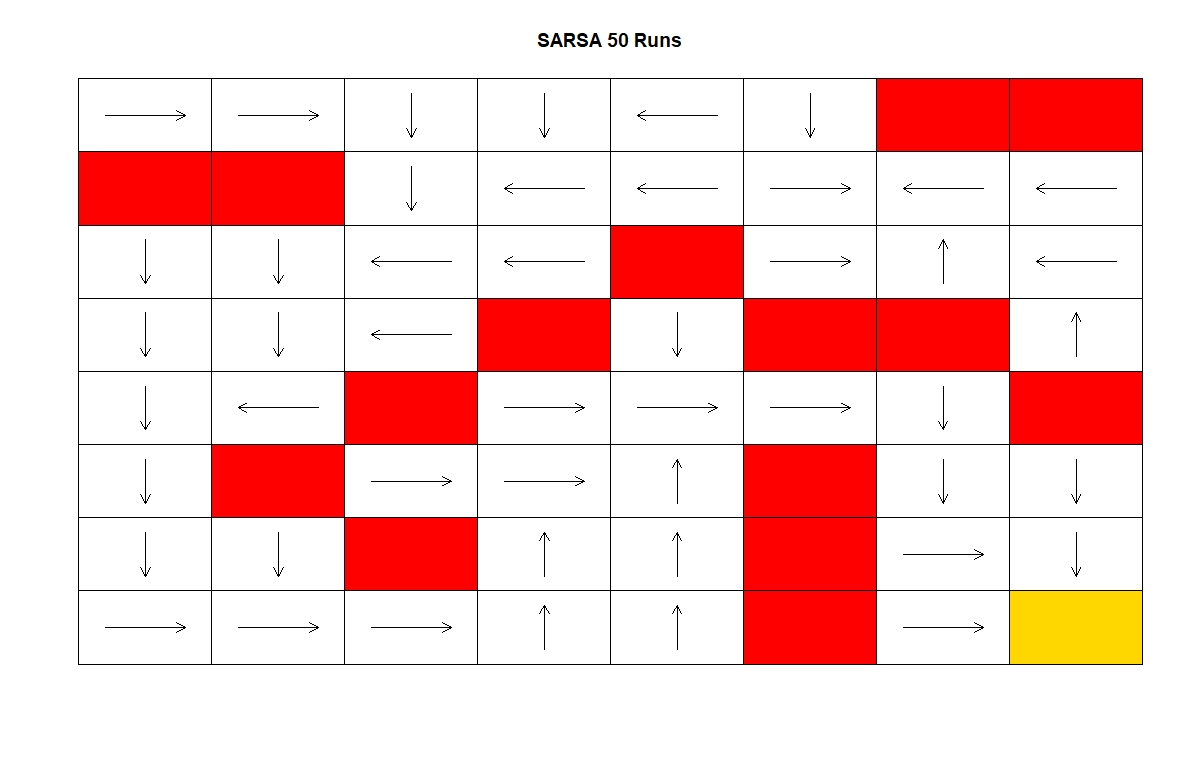
\includegraphics[width=9cm]{figures/Maps/Maze1/SARSAMapMaze1.jpeg}
\end{figure}

\begin{figure}[H]
    \centering
    \caption{Optimal actions on maze 1 using Q-Learning}
    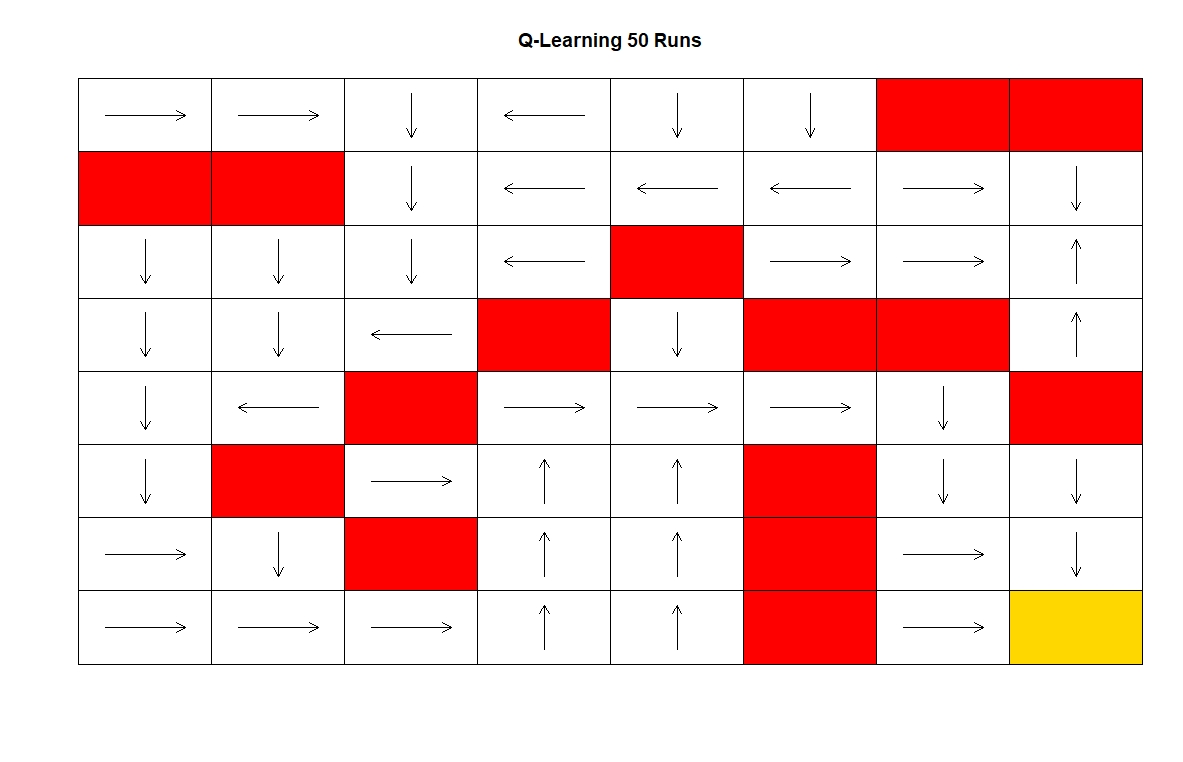
\includegraphics[width=9cm]{figures/Maps/Maze1/QLearningMapMaze1.jpeg}
\end{figure}

\begin{figure}[H]
    \centering
    \caption{Optimal actions on maze 1 using SARSA}
    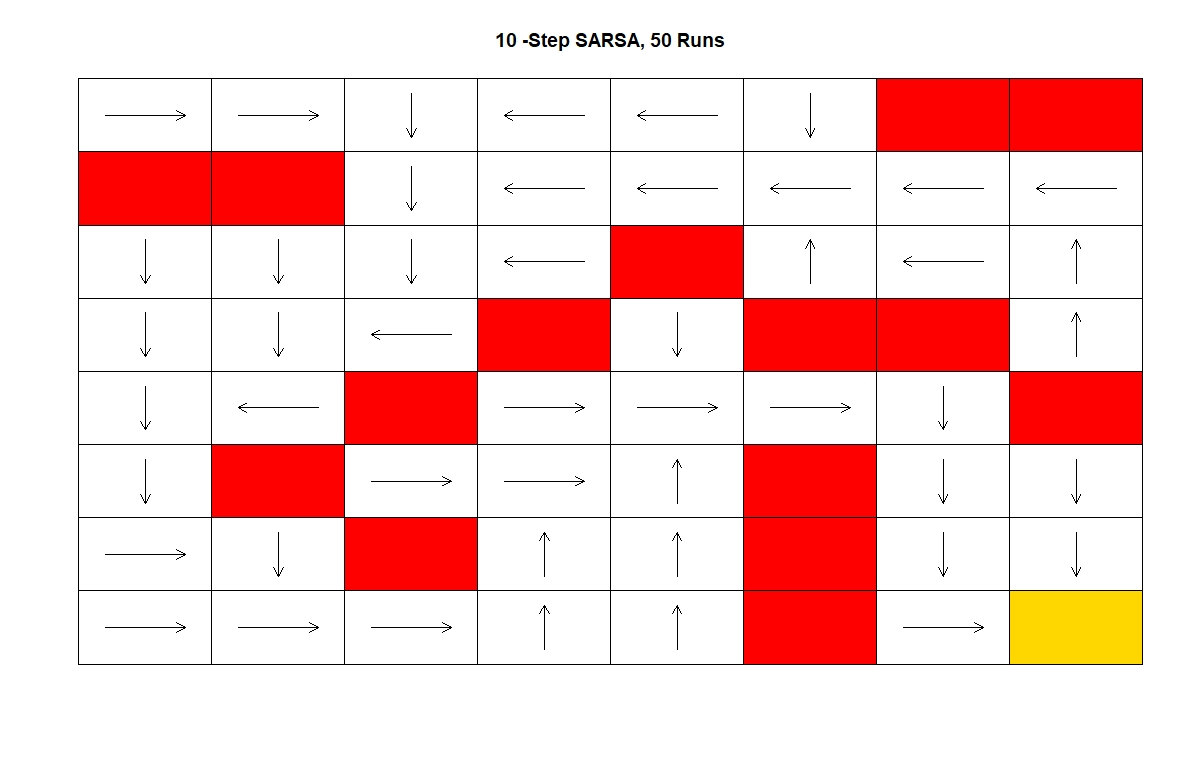
\includegraphics[width=9cm]{figures/Maps/Maze1/10StepSARSAMapMaze1.jpeg}
\end{figure}

\subsection{Maze 2 Results}

\begin{figure}[H]
    \centering
    \caption{Maze 2 returns}
    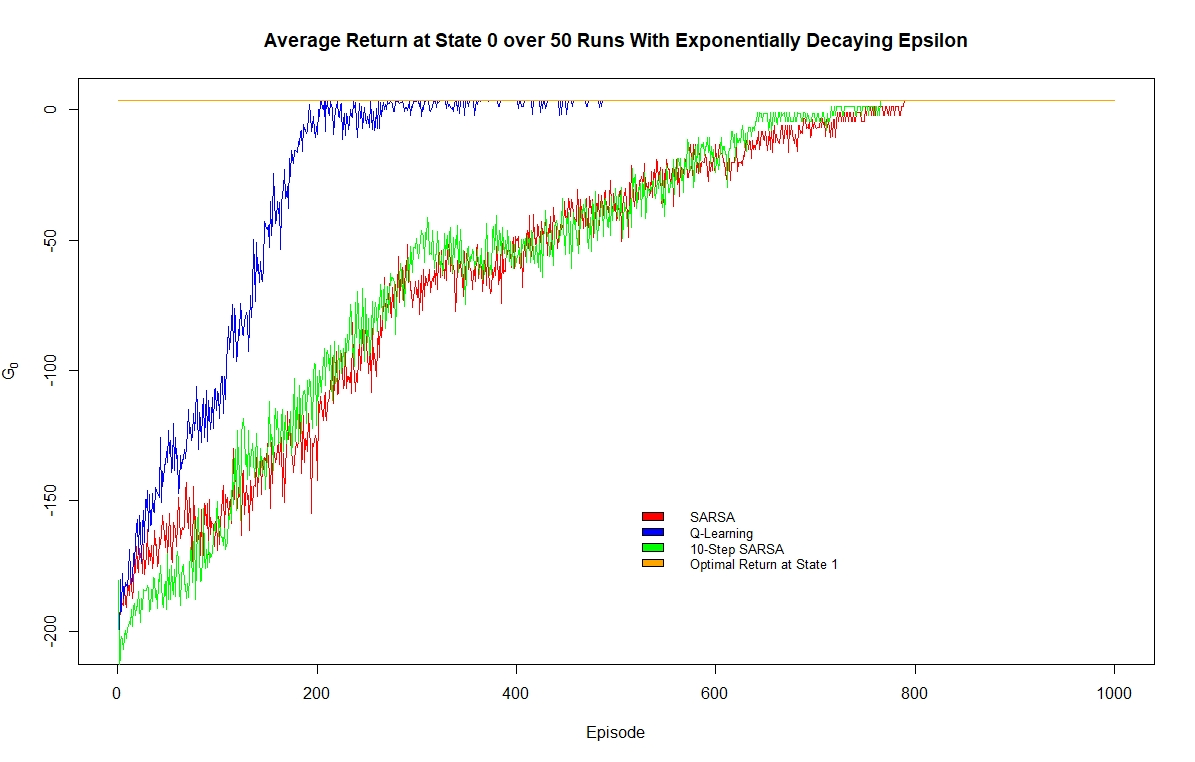
\includegraphics[width=13cm]{figures/Maze2.jpeg}
\end{figure}

\begin{table}[H]
    \centering
    \caption{Maze 2 runtime analysis}
    \begin{tabular}{|c|c|c|}
        \hline
        \textbf{Algorithm} & \textbf{Average \# Episodes Before Convergence} & \textbf{Runtime (mins/run)} \\ \hline
        SARSA & $\sim$800 & $\sim$0.375 \\ \hline
        Q-Learning & $\sim$400 & $\sim$0.275 \\ \hline
        n-Step SARSA & $\sim$800 & $\sim$0.354 \\ \hline
    \end{tabular}
\end{table}

Similar to the plots in maze 1, we observe that Q-Learning converges at a much greater rate than SARSA and 10-step SARSA. It converges in roughly 1/2 the number of episodes and has a per episode runtime approximately 3/4 that of the SARSA algorithms.
\par
In the maze 2 example we are dealing with a $15x15$ grid and therefore a larger discrepancy is to be expected as since there are more states and episodes last longer, the different learning algorithms have a larger room to distinguish themselves from one another.

\begin{figure}[H]
    \centering
    \caption{Optimal actions on maze 2 using Q-Learning}
    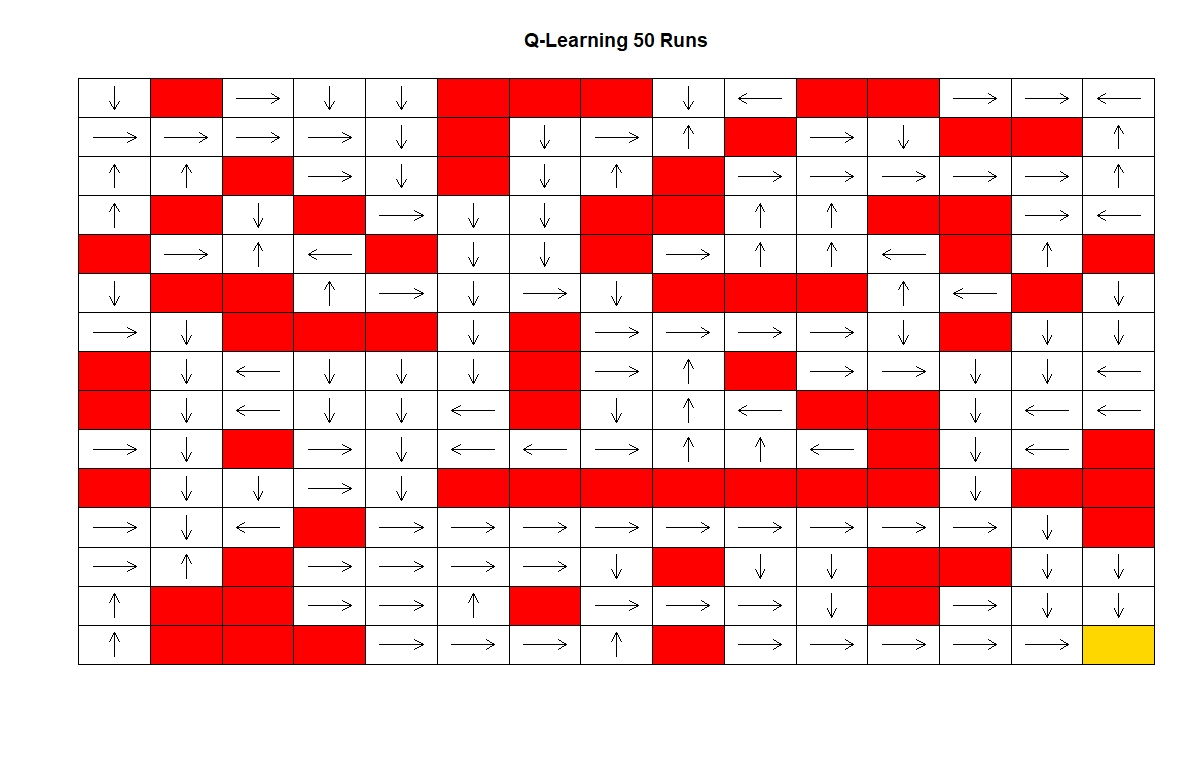
\includegraphics[width=13cm]{figures/Maps/Maze2/QLearningMapMaze2.jpeg}
\end{figure}

\section{Conclusion}

\par
Q-Learning (QL) was the most effective policy based on three factors, scalability, average runtime and average return per policy (or speed to convergence to optimal return per maze). We found that in maze 1, QL converged in $\sim$150 episodes compared to the SARSAs which converged in $\sim$200 episodes with runtimes with an average runtime 0.015min/run slower than QL. For maze 2, which is roughly twice the size of maze 1, the difference became much clearer. QL converged in $\sim$400 episodes compared to the SARSAs which converged in $\sim$800 episodes with runtimes with an average runtime 0.09min/run slower than QL.
\par
A future avenue of research that could benefit our approach would be addressing the issue of not commonly visited states having sub-optimal actions as final optimal actions. This could be solved with the use of deep learning approaches such as neural networks. As in the case of our $8x8$ maze, we see that once the agent found the optimal path, and ceased to explore at the same rate as prior to finding the best route, whatever it had set as the optimal action in some of the states actually isn't optimal. 

\newpage

\section{Appendices}
\subsection{A: Additional Maze 2 Results}

\begin{figure}[H]
    \centering
    \caption{Optimal actions on maze 2 using SARSA}
    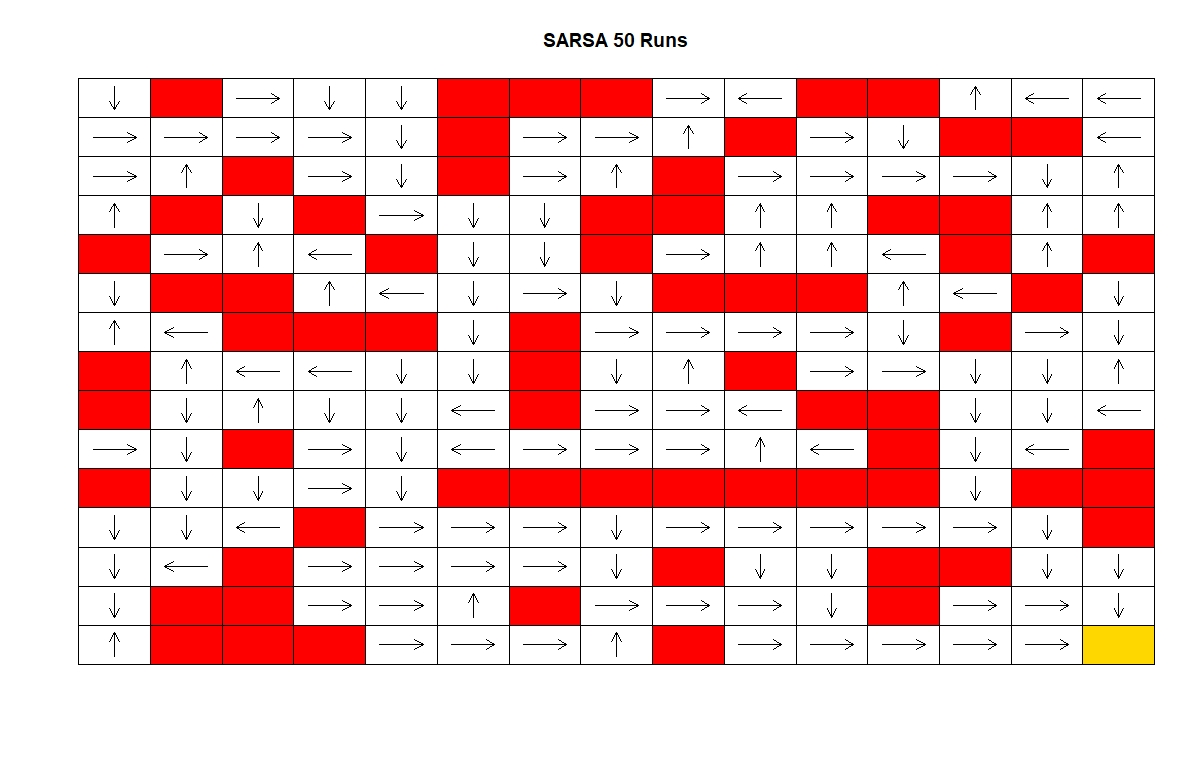
\includegraphics[width=13cm]{figures/Maps/Maze2/SARSAMapMaze2.jpeg}
\end{figure}

\begin{figure}[H]
    \centering
    \caption{Optimal actions on maze 2 using 10-step SARSA}
    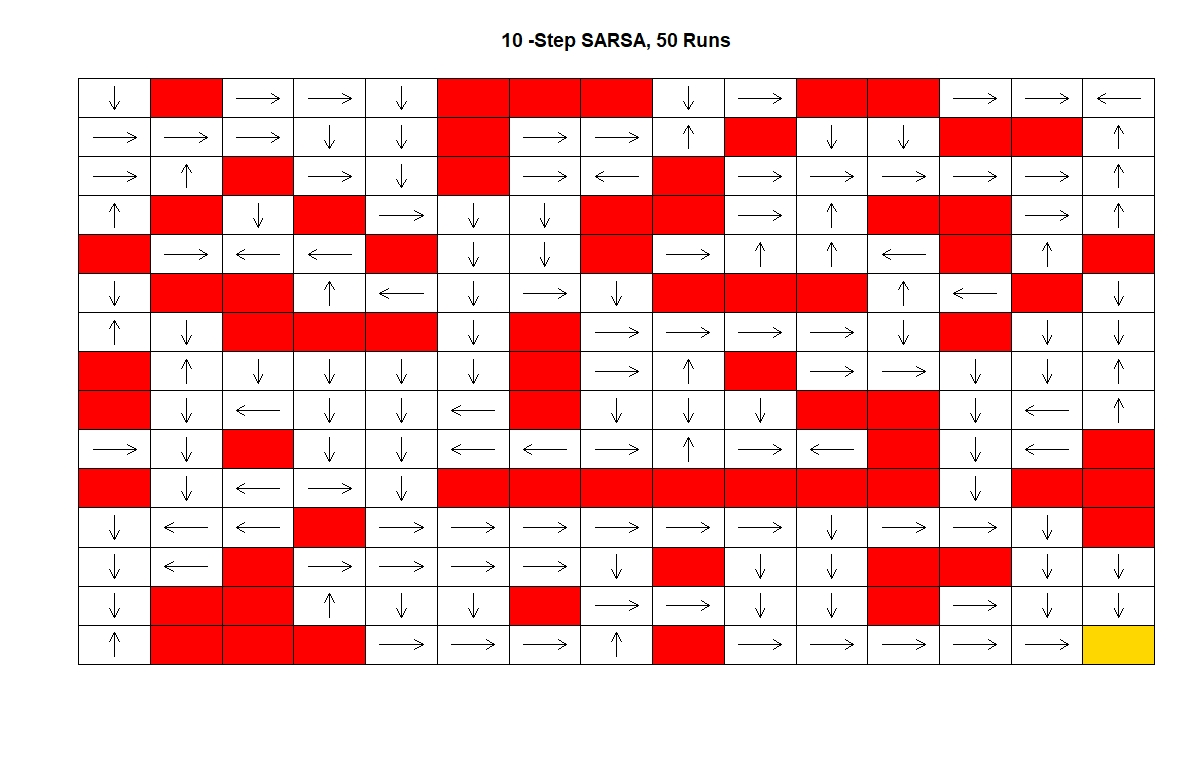
\includegraphics[width=13cm]{figures/Maps/Maze2/10StepSARSAMapMaze2.jpeg}
\end{figure}



\subsection{Appendix B: Choice of Rewards}

In an attempt to accelerate the convergence to $V_{*}(S_0)$, we decided to penalize revisiting an already seen state more severely than visiting an unseen state. The idea is that the agent has more incentive to explore different paths instead of wasting time visiting states it has already seen. We realize this could lead to the agent taking “detours” (i.e., suboptimal actions) to avoid the costly reward of visiting an already seen state. This could explain the suboptimal action choices for states rarely visited (e.g.: in the upper-right part of maze1). However, for states visited sufficiently often, this choice of rewards does not present a problem as demonstrated by the convergence of our algorithms. 

Below we present the results of the algorithms (with an exponentially decaying epsilon) when we set both the reward of visiting an unseen tile and a seen tile to -0.05. We see that the agent finds the optimal action for almost all states; however, convergence to $V_{*}(S_0)$ is slower compared to penalizing the agent for visiting states that it has already seen before. This can be illustrated when comparing figure 5 with figure 14; for Q-Learning, the former reaches optimality at $\sim$150 episodes while the latter reaches optimality at $\sim$200 episodes. Since we are only interested in the convergence rate of $V_{*}(S_0)$, are choice of rewards is further justified. 

\begin{figure}[H]
    \centering
    \begin{minipage}{.33\textwidth}
      \centering
      \caption{SARSA with $r=-0.05$}
      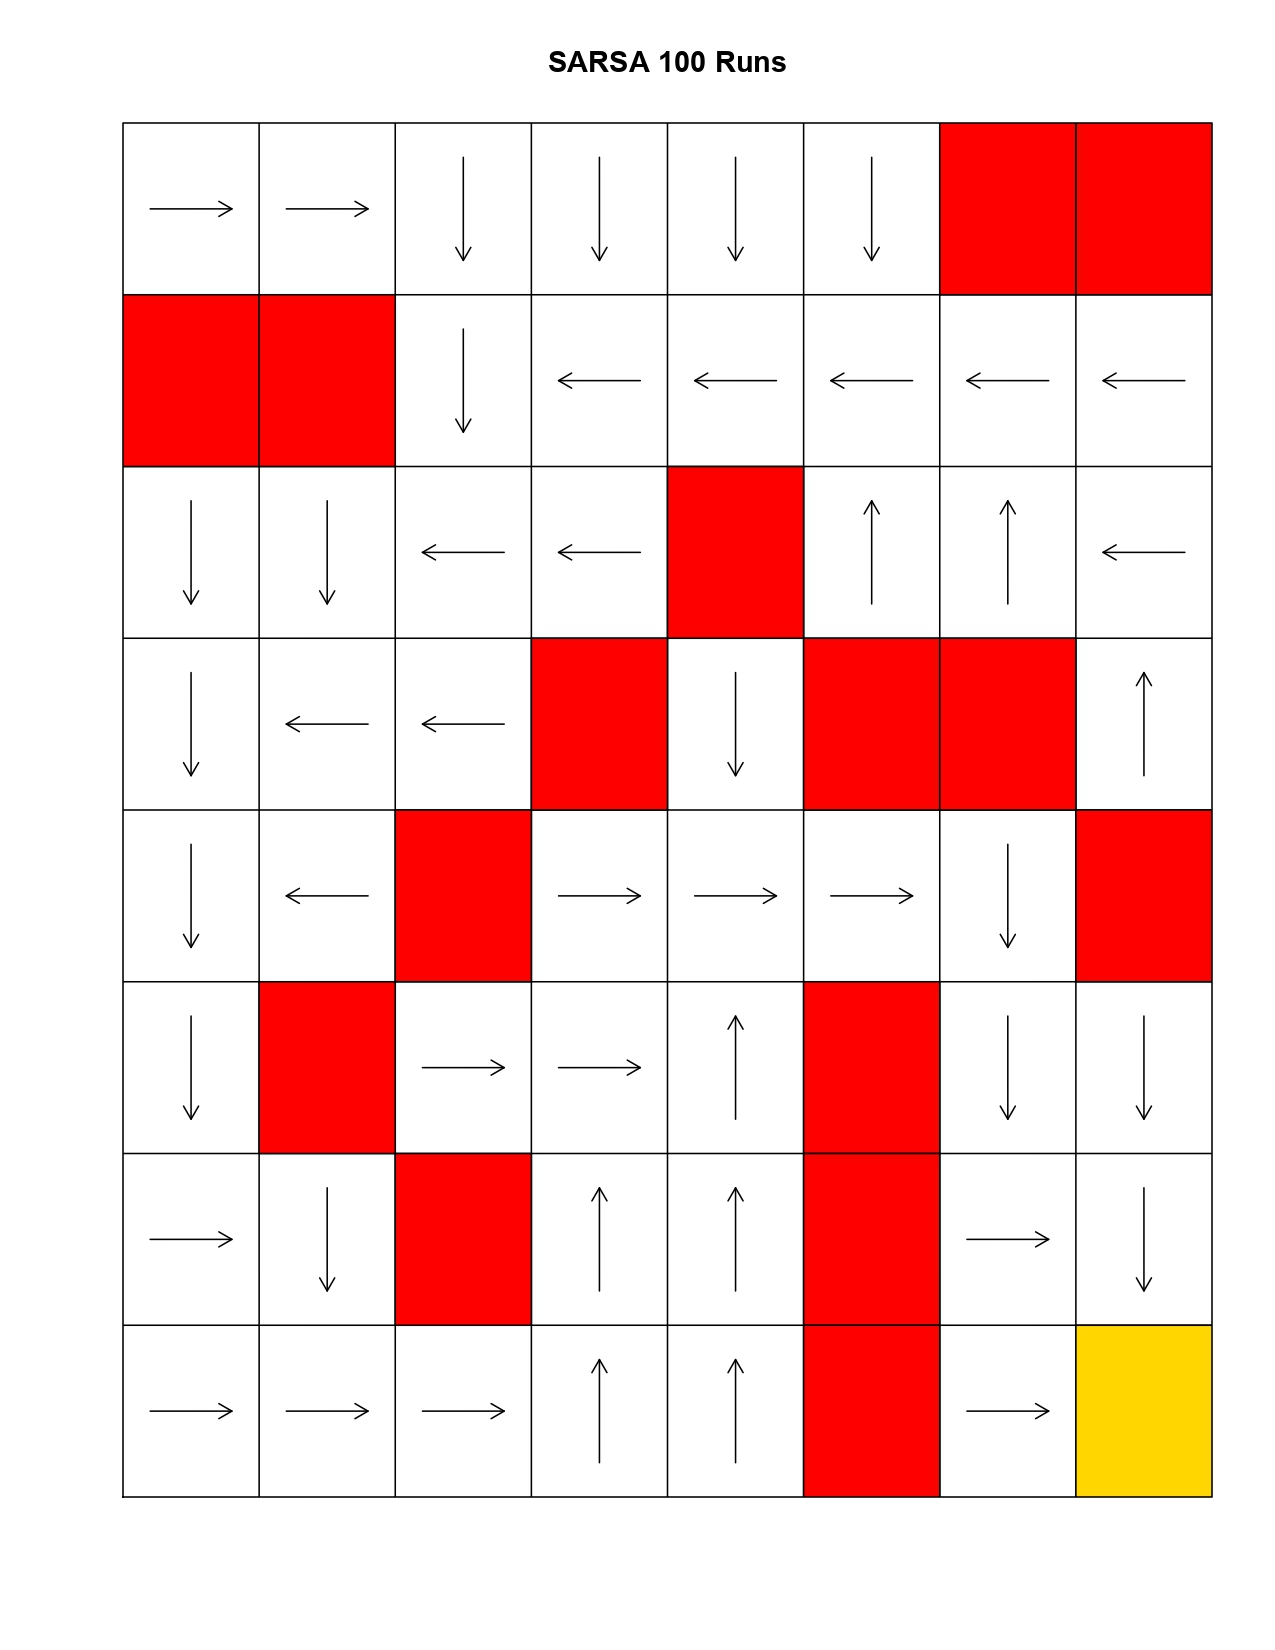
\includegraphics[width=5cm]{figures/005-sarsa.jpg}
    \end{minipage}%
    \begin{minipage}{.33\textwidth}
      \centering
      \caption{QL with $r=-0.05$}
      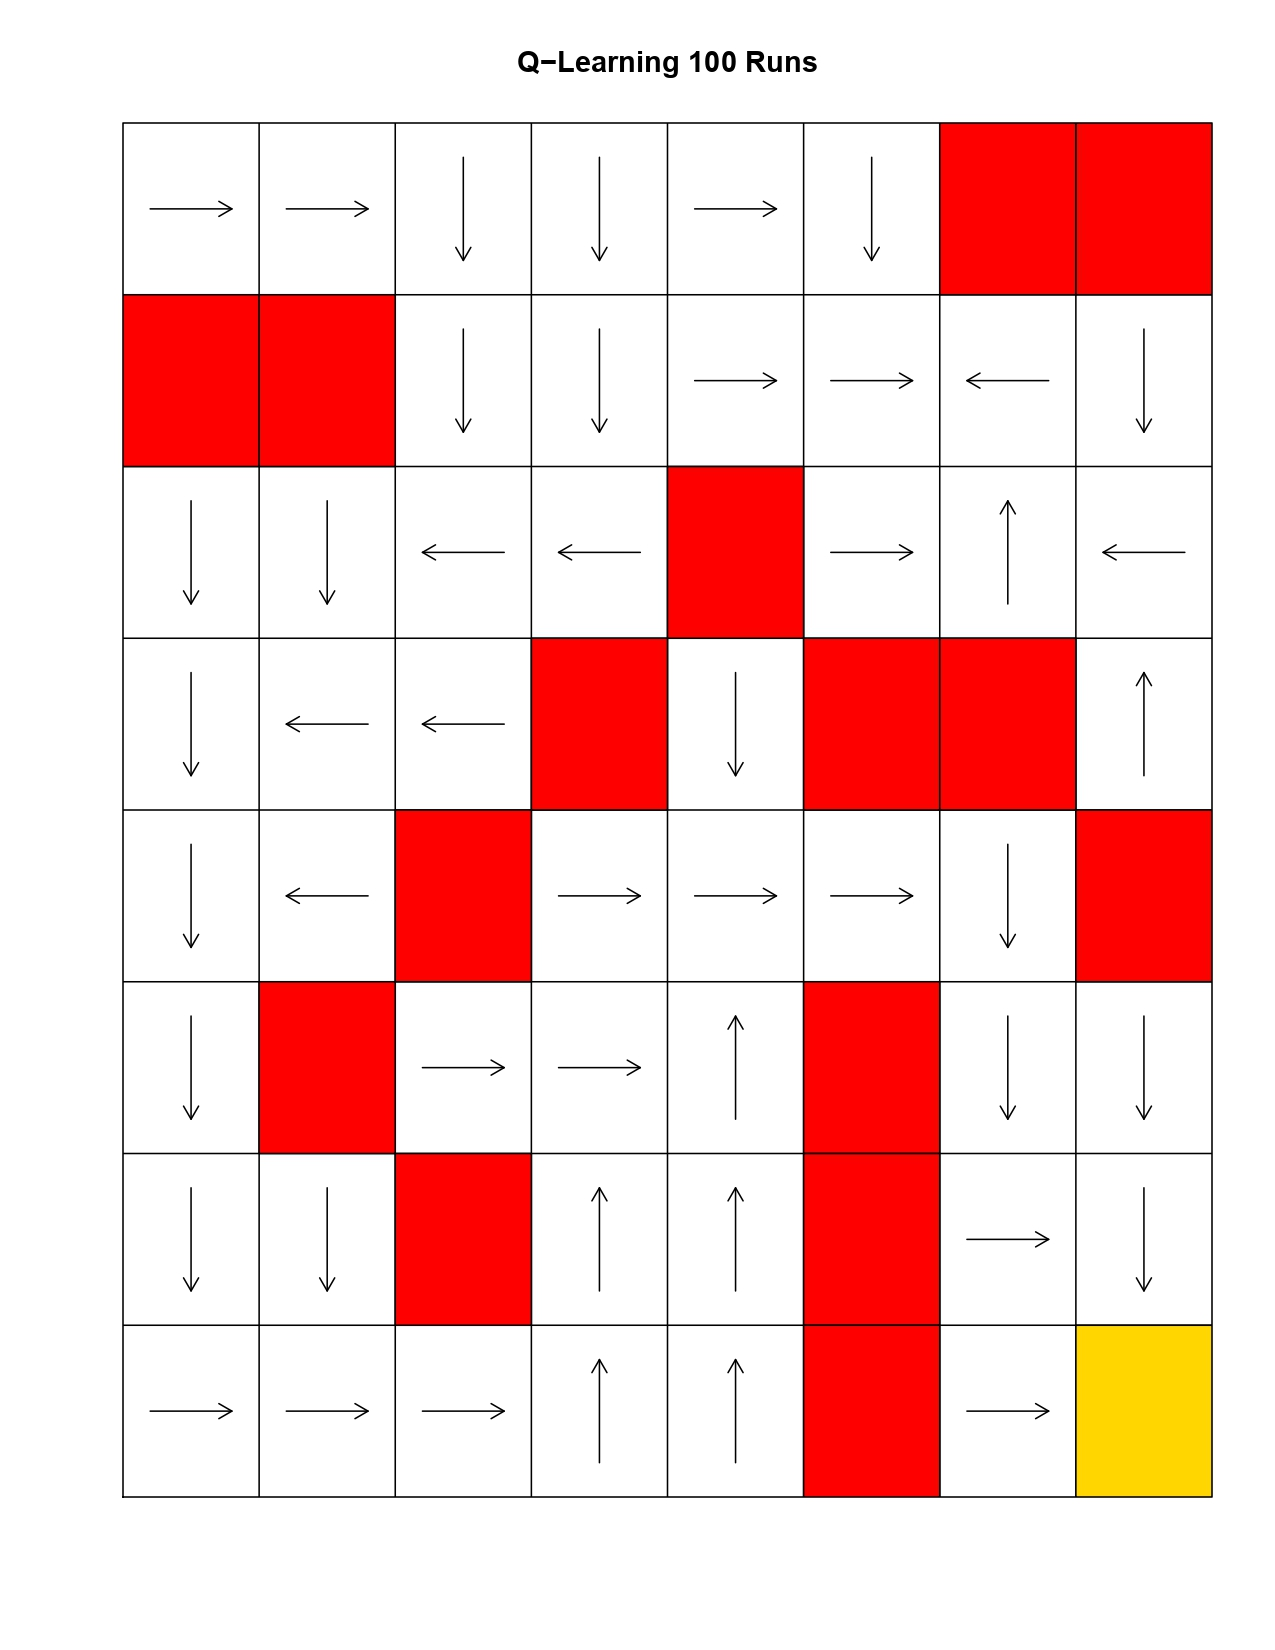
\includegraphics[width=5cm]{figures/005-ql.jpg}
    \end{minipage}
    \begin{minipage}{.33\textwidth}
      \centering
      \caption{10-step SARSA with $r=-0.05$}
      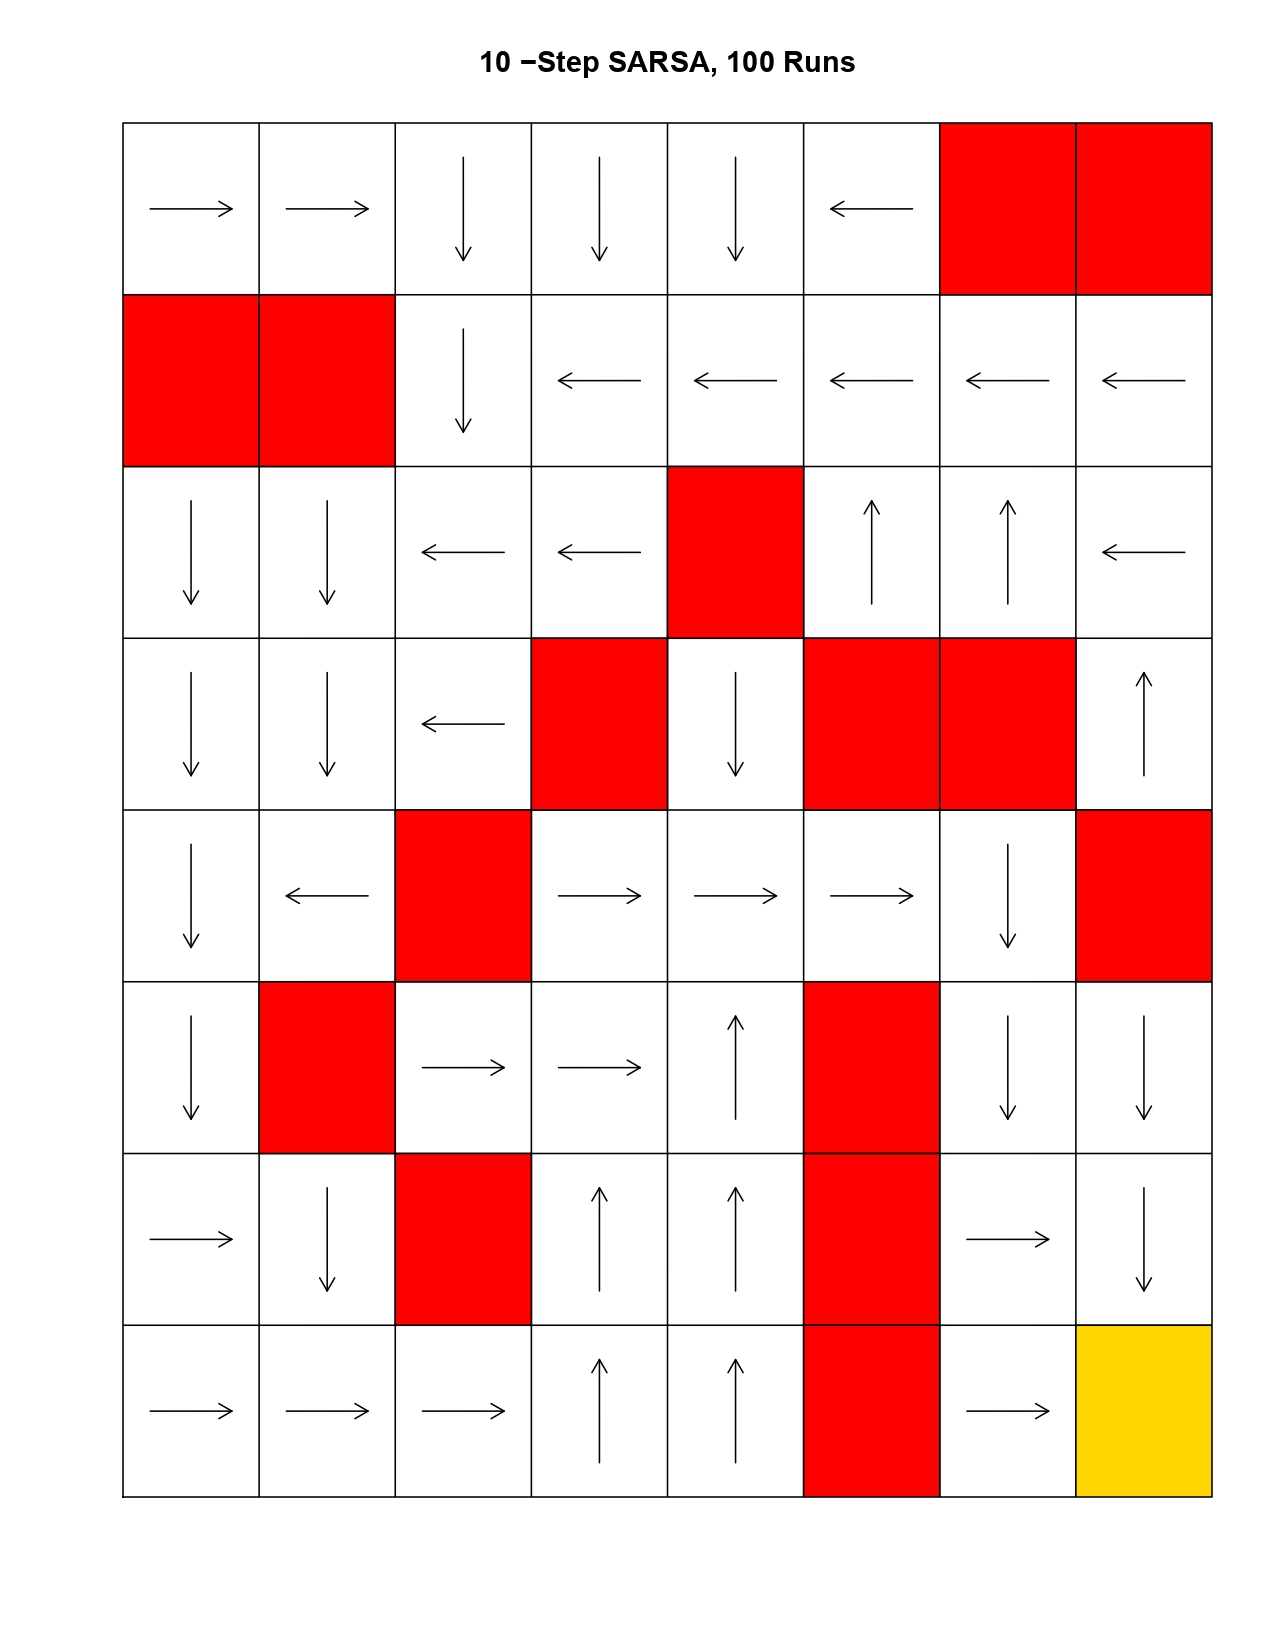
\includegraphics[width=5cm]{figures/005-10sarsa.jpg}
    \end{minipage}
\end{figure}

\begin{figure}[H]
    \centering
    \caption{Average return at state 1 over 50 runs with exponentially decaying epsilon using a constant reward for seen and unseen states.}
    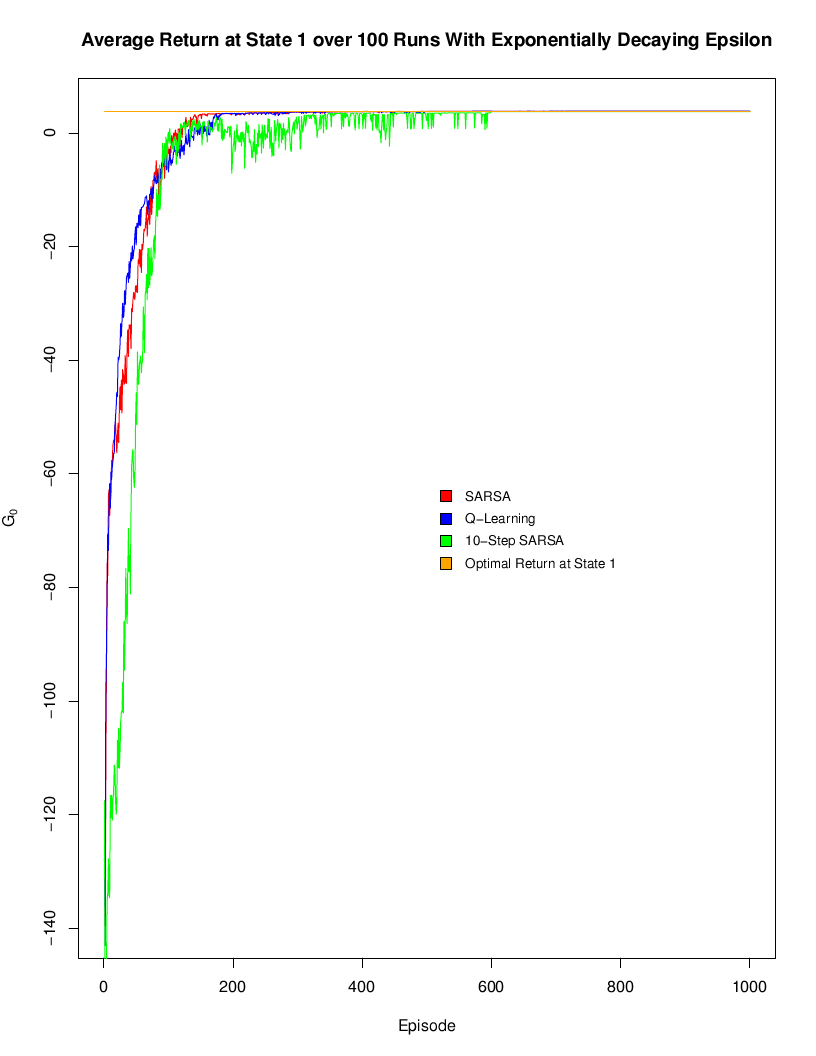
\includegraphics[trim=0 0 0 2cm, clip, width=14cm]{figures/minus005reward.png}
\end{figure}



% Bibliography
\bibliographystyle{elsarticle-num}
\bibliography{refs}

\end{document}
